%%
% 今時jarticleやjbook使ってる人いる?時代はjsarticleかjsbookだよ
% ついでに言うと、uplatexってのはplatexの上位互換、これを使わないなんて旧世代だよね
%
\documentclass[uplatex, report, a4j, 10pt]{jsbook}


%%
% パッケージ群
%
\usepackage{miyazaki-u-paper}   % 宮崎大学工学部の卒論の基本(片山先生作)を、僕がちょっと書き換えちゃった(テヘッ
\usepackage{enumitem}           % enumerate?古い古い
\usepackage[dvipdfmx]{graphicx,hyperref} % 当然dvipdfmなんて使ってないよね
\usepackage{graphicx}
\usepackage[dvipdfmx]{color}    % listingsを使うときにはこれも必須、dvipdfmxを変えちゃうとgraphicxのdvipdfmxも変わるよ
\usepackage{pxjahyper}
\usepackage{listings, jlisting} % コードを埋め込むなら必須
\usepackage{txfonts}            % フォントといえばやっぱりtxfonts、今はnewtxってのもあるらしい
\usepackage{verbatim}           % コメントアウトしてくれる便利なプリアンブルが使える \begin{comment} ... \end{comment}
\usepackage{url}
\usepackage{enumitem}
\usepackage{pdfpages}
% \setlistdepth{6}
% \renewlist{itemize}{itemize}{10}
\hypersetup{
setpagesize=false,
 bookmarksnumbered=true,%
 bookmarksopen=true,%
 colorlinks=true,%
 linkcolor=black,
 citecolor=black,
}
% \usepackage{easy-todo}
\usepackage[hdivide={21mm, , 21mm}, vdivide={30mm, , 25mm}]{geometry} % スタイルを少し変えたくても\hoffset, \voffsetは使わないでね

% todoコマンドを追加
\newcommand\todo[1]{\PackageWarning{Todo}{Detection TODO:#1}\textcolor{red}{(TODO:#1)}}


\renewcommand{\lstlistingname}{コード}
\lstset{
  language={Java},
  frame=tlBR,%フレーム線の指定,上右下左の順,大文字は二重線
%  frameround=tttt,%角の指定,右上|右下|左下|左上の順,tは丸角,fは四角
  framesep=5pt,%本文からframeまでの間隔
  framerule=.2pt,%線の太さ
%  rulecolor={\color[gray]},%線の色
%  backgroundcolor={\color[gray]{.9}},%背景色の指定
  basicstyle={\scriptsize\ttfamily \color[gray]{.15}},%書体の指定,この場合は7ptのタイプライタ体
  identifierstyle={\ttfamily},%識別子の書体
  keywordstyle={\ttfamily \color[cmyk]{0,1,0,0}},%言語ワードの書体
  stringstyle={\scriptsize\ttfamily \color[rgb]{0,0,1}},%文字列リテラルの書体
  commentstyle={\itshape \color[cmyk]{1,0,1,0}},%コメントの書体
  numberstyle={\scriptsize},%行番号の書式
  stepnumber=1,%行番号のステップ間隔
  numbers=left,%行番号の位置
  numbersep=1em,%本文との間隔
  breaklines=true,%改行の設定
  xleftmargin=0zw,
  xrightmargin=0zw,
  columns=[l]{fullflexible},
  lineskip=-0.5zw,
  morecomment={[s][{\color[cmyk]{1,0,0,0}}]{/**}{*/}},
  floatplacement=t,
  classoffset=1,
  showstringspaces=false,%空行の表示
%  breakatwhitespace=true,
%  tabsize=5,
}

\lstdefinestyle{g4}{
  language={C},
  frame=tlBR,%フレーム線の指定,上右下左の順,大文字は二重線
%  frameround=tttt,%角の指定,右上|右下|左下|左上の順,tは丸角,fは四角
  framesep=5pt,%本文からframeまでの間隔
  framerule=.2pt,%線の太さ
%  rulecolor={\color[gray]},%線の色
%  backgroundcolor={\color[gray]{.9}},%背景色の指定
  basicstyle={\scriptsize\ttfamily \color[gray]{.15}},%書体の指定,この場合は7ptのタイプライタ体
  identifierstyle={\ttfamily},%識別子の書体
  keywordstyle={\ttfamily \color[cmyk]{0,1,0,0}},%言語ワードの書体
  stringstyle={\scriptsize\ttfamily \color[rgb]{0,0,1}},%文字列リテラルの書体
  commentstyle={\itshape \color[cmyk]{1,0,1,0}},%コメントの書体
  numberstyle={\scriptsize},%行番号の書式
  stepnumber=1,%行番号のステップ間隔
  numbers=left,%行番号の位置
  numbersep=1em,%本文との間隔
  breaklines=true,%改行の設定
  xleftmargin=0zw,
  xrightmargin=0zw,
  columns=[l]{fullflexible},
  lineskip=-0.5zw,
  morecomment={[s][{\color[cmyk]{1,0,0,0}}]{/**}{*/}},
  floatplacement=t,
  classoffset=1,
  showstringspaces=false,%空行の表示
%  breakatwhitespace=true,
%  tabsize=5,
}


% \lstset{language = modelica,
%         basicstyle=\fontsize{9pt}{10.5pt}\ttfamily,
%         backgroundcolor={\color[gray]{.90}},
%         breakindent = 10pt
%         }
%%
% miyazaki-u-paper.sty用設定値
%
\degree{g} % Graduateのg or Masterのm
\figurenumbering{f} % 図目次を付ける場合はt (真) を持つ真偽値を引数に取る関数
\tablenumbering{f} % 表目次を付ける場合はt (真) を持つ真偽値を引数に取る関数
\title{OpenModelicaのシミュレーション結果を\\用いたモータ特性表自動生成ツールの試作}
\author{原田 海人}
\nendo{元} % 年度
\advisor{片山 徹郎 教授} % 修論では無視する
\major{情報システム工学科}




\begin{document}
\maketitle


%
% 本文
%
\chapter{はじめに}\label{cha:Introduction}
近年、モータは、エアコン・洗濯機・掃除機などの家電製品をはじめ、自動車関係、医療関係など様々な分野に
用いられており\cite{モータ使用製品}、社会に必要不可欠な存在となっている。\\
~はじめに 流れ 案~\\
モータの開発は~で、~の課題がある。それを解決する手段としてシミュレーションがある。
シミュレーションツールの中にOpenModelicaがある。OpenModelicaは~で、~する。
また、結果を画面所にプロットすることで結果を確認できる。
シミュレーションを行った場合、期待通りか結果と比較する。\\
比較する際は、シミュレーション結果から目的のグラフや値を計算等して作成しなければならない。\\
しかし、OpenModelicaではグラフでしか確認できず、具体的な値を取得することが困難である。
そこで、本研究では、モータのシミュレーションをOpenModelicaで行った際のシミュレーション結果の確認にかかる手間を削減することを目的として、
シミュレーション結果のcsvファイルからモータ特性表を自動生成するツールを試作する。\\
% 今回試作したツールで、グラフや値を作成する手間を省くことで、モータ開発の効率化を図る。\\



本論文の構成は、以下の通りである。\\
第2章では、モータ特性表自動生成ツールを試作するために必要となる前提知識について説明する。\\
第3章では、試作したモータ特性表自動生成ツールの構成及び手順について説明する。\\
第4章では、試作したモータ特性表自動生成ツールが正しく動作することを検証する。\\
第5章では、試作したモータ特性表自動生成ツールについて考察する。\\
第6章では、、本論文のまとめとの課題を述べる。\\
\chapter{研究の準備}\label{cha:Preparation}
本章では、本研究で必要となる前提知識を説明する。

\section{モータ作成}\label{motor}
\subsection{仕様書}\label{siyo}
\subsection{シミュレータの役割}\label{simu}

\section{モータ特性表}\label{toku}
\subsection{特性表の種類}\label{syurui}
\subsection{特性表の要素}\label{element}

\section{OpenModelica}\label{OM}

\section{modelica}\label{modelica}



% \section{モータ特性表}\label{win_ap}
% WindowsAPIとは、Windowsプログラミングを行うためにMicrosoftが提供しているAPIのことである[10]。
% APIとはApplication Programming Interfaces の略で、プログラムからソフトウェアを操作するためのインターフェイスのことである[11]。
% WindowsAPIを使用することによって、Windowsアプリを作成するために必要な機能を自ら実装せずにすむので、作業工数を短縮できる[10]。
% 本研究では、ボタンの自動入力などの機能を実装する際に使用した。表2.1に、今回使用する関数を示す。

% \begin{table}[t]
% 	\begin{center}
%   \caption{使用している関数一覧}
%   \begin{tabular}{|l|c|r||r|} \hline
%     関数名 & 説明  \\ \hline \hline
%        GetClientRect & ウィンドウのクライアント領域の座標を取得する。\\ \hline
%        GetDC &ディスプレイデバイスコンテキストのハンドルを取得。\\ \hline
%        CreateDIBSection & DIBとDDB用のビットマップを作成する。 \\ \hline
%        CreateCompatibleDC & メモリデバイスコンテキストのハンドルを取得する。 \\ \hline
% 	   GetForegroundWindow & フォアグラウンドウィンドウのハンドルを取得する。 \\ \hline
%        GetWindowText &フォアグラウンドウィンドウの名前を取得する。\\ \hline
%   \end{tabular}
%   \end{center}
% \end{table}

% \section{Visual Studio}\label{visual_studio}
% Visual Studioとは、MicrosoftがリリースしているWindows環境における統合開発環境のことである[12]。
% 複数のプログラミング言語での開発が可能な開発環境で、Visual Studioを用いることによって、Windowsのクライアントアプリケーションや、
% ハンディターミナルなどのアプリケーション、Webアプリケーションを開発できる。
% 本研究では、テスト支援ツールの概観を作成する際にVisual Studioを用いた。

% \section{Unity}
% Unityとは、ユニティ・テクノロジーズ社が提供する、ゲーム開発フレームワークである。2D、3D、VRなどのゲーム開発で利用されている[13]。
% マルチプラットフォームに対応しており、アセットストアが充実しているため、手軽に高クオリティなゲーム制作ができる。
% 本研究では、作成したテスト支援ツールの適用例で使用するゲームの作成に、このフレームワークを採用する。

% \section{パーティクルフィルター}
% パーティクルフィルター(Particle Filter)とは、確率分布に基づく時系列データの予測手法である[14]。
% パーティクルフィルターでは、現状態から起こりうる多数の次状態を、多数のパーティクルを用いて検出する。
% パーティクルフィルターの基本的な操作手順は、以下の通りである。

% \begin{enumerate}
%   \item リサンプリング : 前フレームでの尤度に従って、パーティクルを撒き直す(追跡対象の周りにパーティクルをばら撒く)。
%   \item 推定 : 等速直線運動や適当な乱数を使い、現フレームにおける追跡対象の位置を推定し、パーティクルを少し動かす。
%   \item 観測 : 現フレームにおける各パーティクルの尤度と重み(正規化)を計算する。つまり、推定の答え合わせをして実際の追跡対象の位置に近いパーティクルの重みを大きくする。
%   			   重みが大きいパーティクルが集中している領域が追跡対象となる。
% \end{enumerate}
% 本研究では、この手法を、キャラクターとオブジェクトの重なり判定に使用する。

% \section{DLL}
% DLL(ダイナミックリンクライブラリ)とは、動的リンクを使ったライブラリである[15]。
% 本研究では、DLLを使うことで、C\#のコードからC++で記述した関数を呼び出す。



\chapter{モータ特性表自動生成ツール}\label{cha:Tool}
本章では、 本研究で試作するモータ特性表自動生成ツールについて説明する。
モータ特性表自動生成ツールは、モータのシミュレーション結果から、\ref{mortoku}節で述べたモータ特性表を自動生成する。
モータ特性表自動生成ツールの処理の流れを、図\ref{fig:kouzou}に示す。
\begin{figure}[t]
	\centering
	% \includegraphics[width=16.5cm]{./Image/.png}
	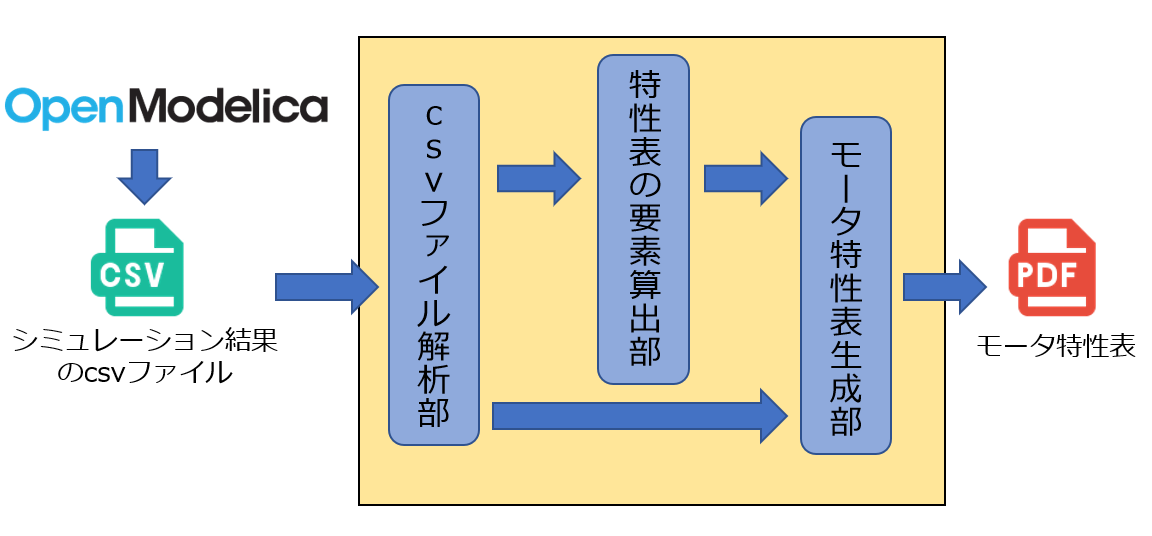
\includegraphics[width=14cm]{./Image/kouzou.png}
    \caption{モータ特性表自動生成ツールの構造}
	\label{fig:kouzou}
  \end{figure}
モータ特性表自動生成ツールの入力は、モータに関してシミュレーションしたOpenModelicaから出力されるcsvファイルである。ここで、現時点のツールは、入力となるcsvファイルは
次の3つの制約をすべて満たす必要がある。
\begin{itemize}
    \item \ref{taioumodel}節で述べたモデルを対象とする
    \item モータの回路に印加する電圧値は一定とする
    \item 0秒からモータに入力を与える
\end{itemize}


モータ特性表自動生成ツールは、3つの処理部で構成しており、それぞれ以下の処理を行う。
\begin{itemize}
    \item csvファイル解析部
    \begin{itemize}
        \item 実行コマンドの取得
        \item csvファイルの読み込み
    \end{itemize}
    \item 特性表の要素算出部
    \begin{itemize}
        \item 基礎データの算出
        \item 特性表の構成要素の算出
    \end{itemize}
    \item モータ特性表生成部
    \begin{itemize}
        \item 特性表の生成
        \item 特性グラフの生成
        \item モータ特性表の生成
    \end{itemize}
\end{itemize}
以下に、それぞれの処理部について説明する。
\section{csvファイル解析部}\label{csv_sec}
csvファイル解析部では、モータ特性表自動生成ツールを実行する際のコマンドから、読み込むcsvファイルを決定する。
そして、指定したcsvファイルを読み込み、モータ特性表を生成するために必要なデータを取得する。
以下に、各処理について説明する。
\subsection{モータ特性表自動生成ツールの実行}\label{sub:zikkou_tool}
読み込むcsvファイルを決定するために、モータ特性表自動生成ツールを実行するコマンドの引数に、ファイル名を指定する。
モータ特性表自動生成ツールを実行するためのコマンドを、コード\ref{code:zikkou}に示す。
\begin{figure*}[t]
	\lstinputlisting[label={code:zikkou}, caption={実行コマンド}]{Image/comand.txt}
\end{figure*}
なお、このコマンドは、ツールの実行ファイルが存在するディレクトリで実行する必要がある。

第1引数には、入力とするcsvファイルのパスを含めたファイル名を指定する。

第2引数には、第1引数で指定したcsvファイルの中の、モータ特性表を自動生成したいモータのモデルに含まれる、慣性部品のオブジェクト名を指定する。

第3引数には、第1引数で指定したcsvファイルの中の、モータ特性表を自動生成したいモータのモデルに含まれる、電源部品のオブジェクト名を指定する。

第2引数と第3引数に、慣性部品と電源部品のオブジェクト名を指定する理由については、\ref{sub:csv_scan}節で述べる。

引数を取得するために、実行コマンドの引数を、1次元の配列で保持するsysライブラリのargvを使用する。
以下に、処理の流れを示す。

\begin{enumerate}
    \item argvの要素数を取得する
    \item 要素数が4以外であれば、図\ref{fig:error_hikisuu}のエラーを表示し、全体の処理を終了する
    \item argvの1番目の要素からcsvファイル名を取得する
    % \item 取得したファイル名の拡張子がcsvでない場合、図\ref{fig:error_file}のエラーを表示し、全体の処理を終了する
    \item argvの2番目の要素から慣性部品のオブジェクト名を取得する
    \item argvの3番目の要素から電源部品のオブジェクト名を取得する
    \item 取得したcsvファイル名、慣性部品のオブジェクト名、電源部品のオブジェクト名をもとに\ref{sub:csv_scan}節で述べる処理を実行する
\end{enumerate}

\subsection{csvファイルの読み込み}\label{sub:csv_scan}
モータ特性表の要素を算出するために必要なデータを、csvファイルから取得する。
今回、モータ特性表の自動生成に必要となるデータの導出計算式は、以下の通りである。
% \vspace{3zh}
\begin{itemize}

    \item 入力
    \begin{eqnarray}
        \mbox{入力 $(\mathrm{W})$} = \mbox{電圧値 $(\mathrm{V})$} \times \mbox{電流値 $(\mathrm{A})$}  \label{siki:in}
    \end{eqnarray}
    \item 出力 
    \begin{eqnarray}
        \mbox{出力 $(\mathrm{W})$} = \mbox{ 負荷トルク $(\mathrm{N \cdot m})$} \times \mbox{角速度 $(\mathrm{rad/s})$} \label{siki:out}
    \end{eqnarray}
    \item 効率
    \begin{eqnarray}
        \mbox{効率 (\%)} = \frac{\mbox{出力 $(\mathrm{W})$}}{\mbox{入力 $(\mathrm{W})$}}  \times 100 \label{siki:effi}
    \end{eqnarray}
    \item 回転数
    \begin{eqnarray}
        \mbox{回転数 $(\mathrm{rpm})$} = \frac{60 \times \mbox{角速度 $(\mathrm{rad/s})$}}{2\pi}   \label{siki:speed}
    \end{eqnarray}
    \item 定格出力
    \begin{eqnarray}
        \mbox{定格出力 $(\mathrm{W})$} = \mbox{最大効率時のトルク $(\mathrm{N \cdot m)}$} \times \mbox{最大効率時の角速度  $(\mathrm{rad/s})$} \times \frac{2\pi}{60} 
        \label{siki:teikaku}
    \end{eqnarray}
     
\end{itemize}

上記の式より、モータ特性表の要素を算出するために必要なデータは、負荷トルク、角速度、電圧、電流である。
また、負荷トルク、角速度、電圧、電流の値を持つcsvファイル内の変数名の拡張子を、表\ref{tab:hensuu}に示す。 
\begin{table}[t]
	\centering
	\caption{各データを持つ拡張子}
	\begin{tabular}{|c|c|} \hline
	  必要なデータ & 変数名 \\ \hline \hline
	  負荷トルク値 & (慣性部品のモジュール名).flange\_a.tau \\ \hline
	  角速度値 &  (慣性部品のモジュール名).w \\ \hline
	  電圧値 &  (電源部品のモジュール名).p.v \\ \hline
	  電流値 &  (電源部品のモジュール名).n.i \\ \hline
	\end{tabular}
	\label{tab:hensuu}
  \end{table}

モータ特性表自動生成ツールで、csvファイルを読み込むために、表\ref{tab:libr}で挙げたcsvライブラリを使用する。csvライブラリを用いた場合、csvファイルを1行ごとに分けて読み込む。
以下に、csvファイルの読み込み処理の流れを示す。
\begin{enumerate}
    \item 取得したファイル名の拡張子がcsvでない場合、図\ref{fig:error_file}のエラーを表示し、全体の処理を終了する
    \item csvファイルを読み込み専用で開く
    \item csvファイルが開けなかった場合、図\ref{fig:error_file}のエラーを表示し、全体の処理を終了する
    \item csvファイルの各行に対して、以下の処理を繰り返す
    \begin{enumerate}
        \item csvファイルから取得した行の各列の値を保持する配列rowに格納する
        \item csvファイルの1行目を読み込んでいる場合、配列rowの要素数分、以下の処理を繰り返す
            \begin{enumerate}
                \item 変数名に、慣性部品のオブジェクト名が含まれている場合、以下の処理を行う
                \begin{enumerate}
                    \item 変数名の末尾に、「.flange\_a.tau」が含まれている場合、その変数名を格納している配列rowのインデックスを取得する
                    \item 変数名の末尾に、「.w」が含まれている場合、その変数名を格納している配列rowのインデックスを取得する
                \end{enumerate}
                \item 変数名に、電源部品のオブジェクト名が含まれている場合、以下の処理を行う
                \begin{enumerate}
                    \item 変数名の末尾に、「.p.v」が含まれている場合、その変数名を格納している配列rowのインデックスを取得する
                    \item 変数名の末尾に、「.n.i」が含まれている場合、その変数名を格納している配列rowのインデックスを取得する
                \end{enumerate}
            \end{enumerate}
            % \item 3.(a)で配列rowのインデックスを4つ取得するが、いずれか1つでも取得できない場合、図\ref{fig:error_comand}のエラーを表示し、全体の処理を終了する
            \item 4.(b)で配列rowのインデックスを4つ取得し、いずれか1つでも取得できない場合、図\ref{fig:error_comand}のエラーを表示し、全体の処理を終了する
  
        % \item csvファイルの2行目を読み込んでいる場合、以下の処理を行う
        % \begin{enumerate}
        %     \item トルク値の0.0秒段階の値を変数 torque\_defaultに代入する
        %     \item 角速度値の0.0秒段階の値を変数 angularvelocity\_defaultに代入する
        %     \item 電圧値の0.0秒段階の値を変数volyage\_defaultに代入する
        %     \item 電流値の0.0秒段階の値を変数 current\_defaultに代入する
        % \end{enumerate}
        \item csvファイルの2行目以下を読み込んでいる場合、以下の処理を行う
        \begin{enumerate}
            \item トルク値を格納する配列 torqueに、4.(b).i.A.で取得した配列rowのインデックスをキーに持つ値を格納する
            \item 角速度値を格納する配列 angularvelocityに、4.(b).i.B.で取得した配列rowのインデックスをキーに持つ値を格納する
            \item 電圧値を格納する配列 voltageに、4.(b).ii.A.で取得した配列rowのインデックスをキーに持つ値を格納する
            \item 電流値を格納する配列 currentに、4.(b).ii.B.で取得した配列rowのインデックスをキーに持つ値を格納する
        \end{enumerate}
    \end{enumerate}

\end{enumerate}
% なお、上記の処理の流れにおいて、
% csvファイルの2行目を読み込まない理由は、\ref{OM}節で述べたように、2行目にはモデルを作成した際の初期値が格納されており、初期値はモータ特性表の要素を算出することに使用しないからである。
\begin{figure}[t]
	\centering
	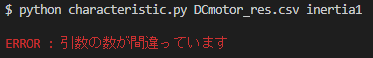
\includegraphics[width=10cm,height=1.5cm]{./Image/error_tarinai.png}
	\caption{引数の数に誤りがあった場合のエラー文の例}
	\label{fig:error_hikisuu}
\end{figure}
\begin{figure}[t]
	\centering
	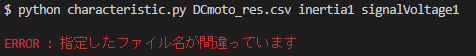
\includegraphics[width=12cm,height=1.5cm]{./Image/error_file.png}
	\caption{第1引数に誤りがあった場合のエラー文の例}
	\label{fig:error_file}
\end{figure}
\begin{figure}[t]
	\centering
	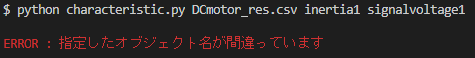
\includegraphics[width=12cm,height=1.5cm]{./Image/error_comand.png}
	\caption{第2引数、第3引数に誤りがあった場合のエラー文の例}
	\label{fig:error_comand}
\end{figure}

\section{特性表の要素算出部}\label{youso_sec}
特性表の要素算出部では、\ref{sub:csv_scan}節で取得したデータをもとに、特性表の各要素を算出する。
まず、特性表の各要素を算出するために必要となる基礎データを算出する。基礎データとは、回転数、出力、効率の値のことを指す。
そして、\ref{sub:csv_scan}節で取得したデータと、基礎データから特性表の各要素を算出する。
以下より、各処理について説明する。

\subsection{基礎データの算出}\label{sub:youso_kiso}
基礎データの算出処理では、回転数、出力、効率の値を持つ配列を、それぞれの値に対して生成する。
各配列の生成方法を以下に示す。以下の式で

\subsubsection{回転数}\label{sub:sub:kaiten}
% 回転数を算出する式は、\ref{sub:csv_scan}節の箇条書き中にある、回転数にて示した式を用いる。
回転数を算出する式は、%\ref{sub:csv_scan}節の
(\ref{siki:speed})式を用いる。
配列angularvelocityの各要素を、それぞれ(\ref{siki:speed})式に適用し、回転数の値を持つ配列speedを生成する。

\subsubsection{出力}\label{sub:sub:syutu}
% 出力を算出する式は、\ref{sub:csv_scan}節の箇条書き中にある、出力にて示した式を用いる。%\ref{sub:csv_scan}節の
% (\ref{siki:out})式を用いて、出力を算出する。
% 配列torqueと、配列angularvelocityの同じインデックスの要素を、(\ref{siki:out})式にあてはめ、出力を算出する。
% 配列torqueと、配列angularvelocityの最後のインデックスの要素までの出力を計算し、配列outputを生成する。
出力を算出する式は、%\ref{sub:csv_scan}節の
(\ref{siki:out})式を用いる。
配列torqueと、配列angularvelocitの各要素を、それぞれ(\ref{siki:out})式に適用し、出力の値を持つ配列outputを生成する。
% 配列torqueと、配列angularvelocityの最後のインデックスの要素までの出力を計算し、回転数の値を持つ配列speedを生成する。
\subsubsection{効率}\label{sub:sub:kouritu}
% 効率を算出する式は、\ref{sub:csv_scan}節の箇条書き中にある、効率にて示した式と入力にて示した式を用いる。
% 効率を算出する式は、%\ref{sub:csv_scan}節の
% (\ref{siki:effi})式を用いて、効率を求める。
% 配列voltageと配列currentと配列outputそれぞれの最初のインデックスの要素を、(\ref{siki:in})式にあてはめ、効率を求める。
% この処理を各配列の最後まで繰り返し、配列efficiencyを生成する。
% また、配列voltageと配列currentのどちらか一方でも「0」だった場合、効率値を「0」とする。これは、0除算を防ぐために行う。
効率を算出する式は、%\ref{sub:csv_scan}節の
(\ref{siki:effi})式を用いる。
配列voltageと配列currentを(\ref{siki:in})式に適用し、入力の値を算出する。算出した入力の値と、配列outputの要素を、(\ref{siki:effi})式に適用し、効率の値を持つ配列efficiencyを生成する。

\subsection{特性表の各要素の算出}\label{sub:youso_mortoku}
特性表の各要素の算出処理では、\ref{sub:tokuseihyou}節で述べた9つの要素を算出する。

\subsubsection{定格電圧}\label{sub:sub:dennatu}
モータ特性表自動生成ツールが対応するモデルでは、電圧値が一定のため、配列voltageの要素はすべて同じ値になる。今回は、0番目の値を定格電圧とする。

\subsubsection{始動電流}\label{sub:sub:sidouden}
始動電流とは、モータの起動時に流れる大きな電流である。モータの起動直後は逆起電力が発生するため、モータ・コイル部分にかかる電圧が下がり、電流値も下がる。
したがって、配列currentの要素の最大値を始動電流とする。

\subsubsection{停動トルク}\label{sub:sub:teidoutoruku}
停動トルクとは、モータが出しうる最大の負荷トルク値である。したがって、配列torqueの要素の最大値を停動トルクとする。

\subsubsection{最大効率}\label{sub:sub:saidaikouritu}
配列efficiencyの要素の最大値を最大効率とする。

\subsubsection{定格トルク}\label{sub:sub:teikakutoruku}
定格トルクとは、最大効率時の負荷トルク値である。まず、配列efficiencyの中で、最大効率である要素のインデックスXを取得する。
そして、配列torqueのインデックスXの要素を定格トルクとする。
% 配列torqueの中で、取得した最大効率のインデックスと同じ位置にある値を定格トルクとする。

\subsubsection{定格回転数}\label{sub:sub:teikakukaiten}
定格回転数とは、最大効率時の回転数の値である。まず、配列efficiencyの中で、最大効率である要素のインデックスXを取得する。
そして、配列speedのインデックスXの要素を定格回転数とする。
% そして、配列torqueのインデックスXの要素を定格トルクとする。
% 配列speedの中で、取得した最大効率のインデックスと、同じ位置にある値を定格回転数とする。

\subsubsection{定格電流}\label{sub:sub:teikakuden}
定格電流とは、最大効率時の電流値である。まず、配列efficiencyの中で、最大効率である要素のインデックスXを取得する。
そして、配列currentのインデックスXの要素を定格電流とする。
% の中で、取得した最大効率のインデックスと、同じ位置にある値を定格電流とする。

\subsubsection{定格出力}\label{sub:sub:teikakusyutu}
定格出力とは、定格動作点における出力の値である。(\ref{siki:teikaku})式を用いて、定格出力を求める。上記で求めた定格トルクと定格回転数を、(\ref{siki:teikaku})式に代入し、
求めた解が定格出力である。
% 定格出力を算出する式は、%\ref{sub:csv_scan}節の
% \ref{siki:teikaku}式を用いる。
% 上記の定格トルクと定格回転数で求めた値を、定格出力を算出する式に代入し、得た値が定格出力である。

\subsubsection{最大回転数}\label{sub:sub:saidaikai}
配列speedの要素の最大値を最大回転数とする。

\section{モータ特性表生成部}\label{mortoku_sec}
モータ特性表生成部では、\ref{csv_sec}節と\ref{youso_sec}節で算出した要素を用いて、モータ特性表を自動生成する。まず、特性表を生成し、画像として保存する。
次に、\ref{sub:tokuseigurahu}節で挙げた4つの特性グラフを生成し、画像として保存する。最後に、特性表の画像と、特性グラフの画像をPDFファイルに書き込むことで、モータ特性表を生成する。
以下に、各処理について説明する。

\subsection{特性表生成}\label{sub:mortortoku}

特性表生成処理では、特性表を生成する。以下に、処理の流れを示す。
\begin{enumerate}
    % \item \ref{sub:youso_mortoku}節で求めたそれぞれの値と、コード\ref{code:name}に示す配列を用いて、特性表を生成する
    \item \ref{sub:youso_mortoku}節で求めたそれぞれの値を、表\ref{tab:wakugumi}にあてはめて、特性表を生成する
    % \item 特性表の各要素の名前を持つ配列を作成する(コード\ref{code:name}参照)
    % \item 特性表の要素の配列と、特性表の各要素の名前を持つ配列から、特性表用の配列を作成する
    \item 生成した表の上部にタイトルとして「モータ特性表」の文字を追加し、画像として保存する。
\end{enumerate}

\begin{table}[t]
	\centering
	\caption{特性表の枠組み}
	\begin{tabular}{|c|c|} \hline
	  要素 & データ \\ \hline \hline
	  定格電圧$(\mathrm{V})$ & \ref{sub:youso_mortoku}節で求めた定格電圧の値 \\ \hline
	  始動電流 $(\mathrm{mA})$&  \ref{sub:youso_mortoku}節で求めた始動電流の値 \\ \hline
	  停動トルク $(\mathrm{mN \cdot m})$& \ref{sub:youso_mortoku}節で求めた停動トルクの値  \\ \hline
      最大効率 $(\mathrm{\%})$& \ref{sub:youso_mortoku}節で求めた最大効率の値  \\ \hline
      定格トルク $(\mathrm{mN \cdot m})$& \ref{sub:youso_mortoku}節で求めた定格トルクの値 \\ \hline
	  定格回転数 $(\mathrm{rpm})$& \ref{sub:youso_mortoku}節で求めた定格回転数の値  \\ \hline
      定格電流 $(\mathrm{mA})$& \ref{sub:youso_mortoku}節で求めた定格電流の値  \\ \hline
      定格出力 $(\mathrm{W})$& \ref{sub:youso_mortoku}節で求めた定格出力の値 \\ \hline
	  最大回転数 $(\mathrm{rpm})$&  \ref{sub:youso_mortoku}節で求めた最大回転数の値 \\ \hline
	\end{tabular}
	\label{tab:wakugumi}
  \end{table}

上記の処理で生成したタイトルと特性表の画像を、図\ref{fig:toku_gazou}に示す。
% \begin{figure*}[t]
% 	\lstinputlisting[label={code:name}, caption={特性表を構成する要素名の配列}]{Image/name.txt}
% \end{figure*}
\begin{figure}[t]
    \centering
    \fbox{
	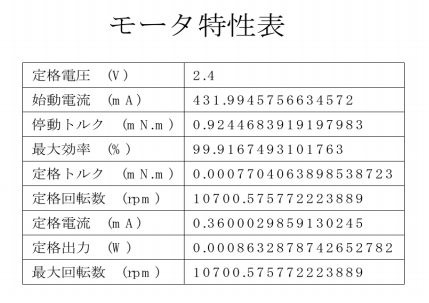
\includegraphics[width=7cm]{./Image/characteristicTable.png}
    }
    \caption{タイトルと特性表の画像}
	\label{fig:toku_gazou}
\end{figure}

\subsection{特性グラフ生成}\label{sub:toku_gurahu}
\ref{sub:csv_scan}節、\ref{sub:youso_kiso}節で求めた要素の配列を用いて、特性グラフを生成する。
処理の流れを以下に示す。
\begin{enumerate}
    % \item 配列torqueに、torque\_defaultを格納する
    % \item 配列currentに、current\_defaultを格納する
    % \item 配列speedに、angularvelocity\_defaultから\ref{siki:speed}式を適用した値を格納する
    % \item current\_defaultが0か判定し、以下の処理を行う
    % \begin{enumerate}
    %     \item 0だった場合、配列efficiencyに、0を格納する
    %     \item 0ではない場合、以下の処理を行う
    %     \begin{enumerate}
    %         \item current\_defaultと、voltage\_defaultを用いて\ref{siki:in}式から、0.0秒段階の入力の値を保持するinput\_defaultに代入する
    %         \item torque\_defaultと、angularvelocity\_defaultを用いて\ref{siki:out}式から、0.0秒段階の出力の値を保持するoutput\_defaultに代入する
    %         \item 配列efficiencyに、input\_defaultと、output\_defaultを\ref{siki:effi}式に適用した値を格納する
    %     \end{enumerate}
    % \item 配列outputに、torque\_defaultと、angularvelocity\_defaultを\ref{siki:out}式に適用した値を格納する
    % \end{enumerate}
    \item x軸に配列torqueを、y軸に配列currentを指定し、ライブラリmatplotlib(表\ref{tab:libr}参照)を用いてグラフを生成し、画像として保存する
    \item 1.の処理に対して、y軸に配列speedを指定した場合、y軸に配列efficiencyを指定した場合、y軸に配列outputを指定した場合を適用し、それぞれグラフを画像として保存する
\end{enumerate}
上記の処理で生成した4つのグラフを、それぞれ図\ref{fig:current}、図\ref{fig:speed}、図\ref{fig:effi}、図\ref{fig:output}に示す。

\begin{figure}[t]
    \begin{tabular}{cc}
        \begin{minipage}{0.45\hsize}
            \centering
            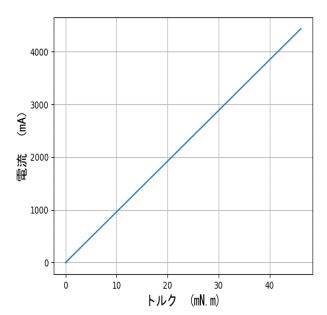
\includegraphics[width=.8\columnwidth]{./Image/current.png}
            \caption{「負荷トルク $\times$ 電流」グラフ}
            \label{fig:current}
        \end{minipage}
        \hfill
        \begin{minipage}{0.45\hsize}
            \centering
            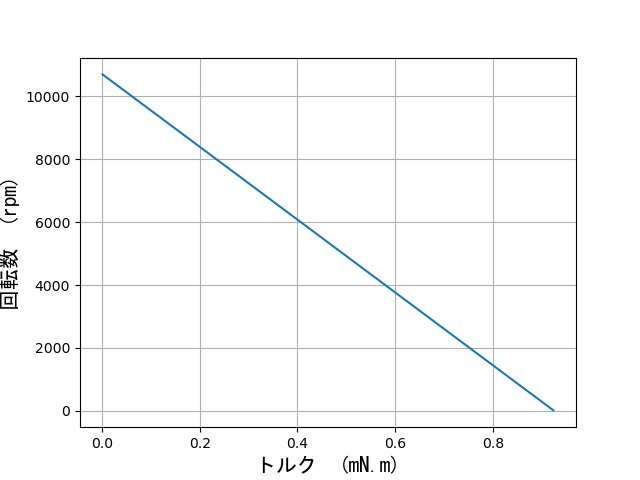
\includegraphics[width=.82\columnwidth]{./Image/speed.png}
            \caption{「負荷トルク $\times$ 回転数」グラフ}
            \label{fig:speed}
        \end{minipage}\\\\
        \begin{minipage}{0.45\hsize}
            \centering
            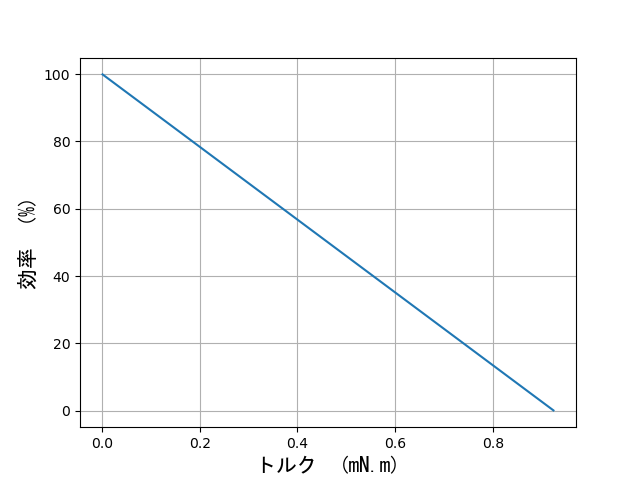
\includegraphics[width=.84\columnwidth]{./Image/efficiency.png}
            \caption{「負荷トルク $\times$ 効率」グラフ}
            \label{fig:effi}
        \end{minipage}
        \hfill
        \begin{minipage}{0.45\hsize}
            \centering
            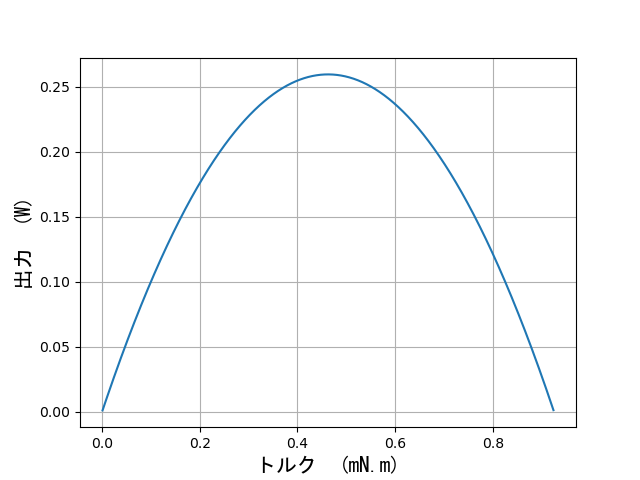
\includegraphics[width=.8\columnwidth]{./Image/output.png}
            \caption{「負荷トルク $\times$ 出力」グラフ}
            \label{fig:output}
        \end{minipage}
    \end{tabular}
\end{figure}
% \begin{figure}[t]
% 	\centering
% 	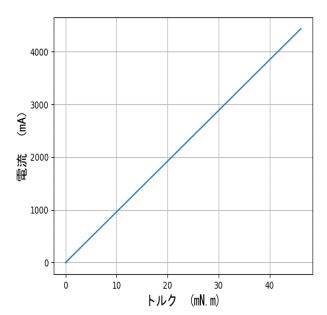
\includegraphics[width=7cm]{./Image/current.png}
% 	\caption{「負荷トルク $\times$ 電流」グラフ}
% 	\label{fig:current}
% \end{figure}
% \begin{figure}[t]
% 	\centering
% 	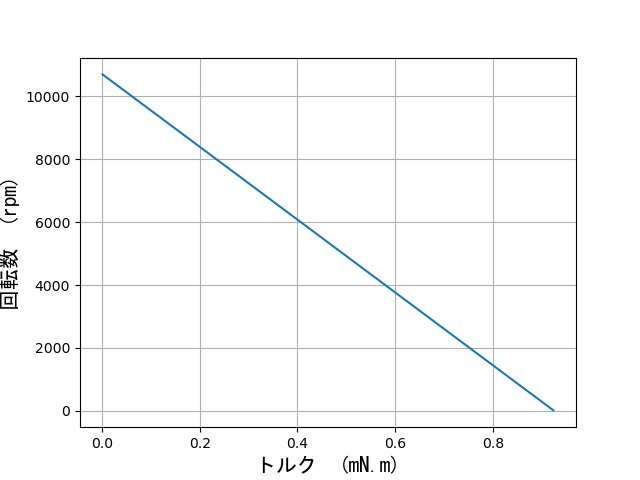
\includegraphics[width=7cm]{./Image/speed.png}
% 	\caption{「負荷トルク $\times$ 回転数」グラフ}
% 	\label{fig:speed}
% \end{figure}
% \begin{figure}[t]
% 	\centering
% 	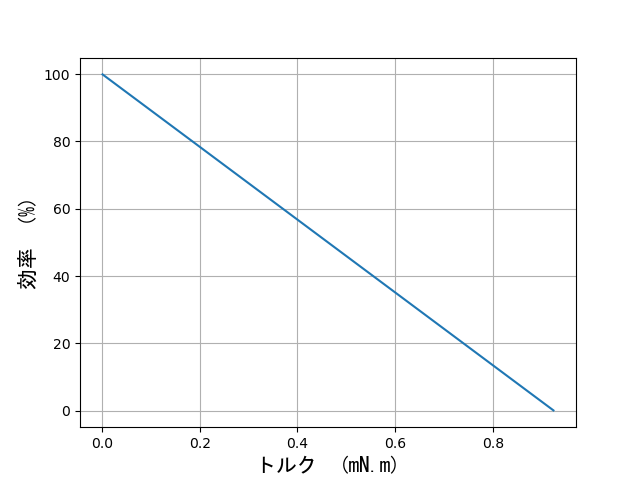
\includegraphics[width=7cm]{./Image/efficiency.png}
% 	\caption{「負荷トルク $\times$ 効率」グラフ}
% 	\label{fig:effi}
% \end{figure}
% \begin{figure}[t]
% 	\centering
% 	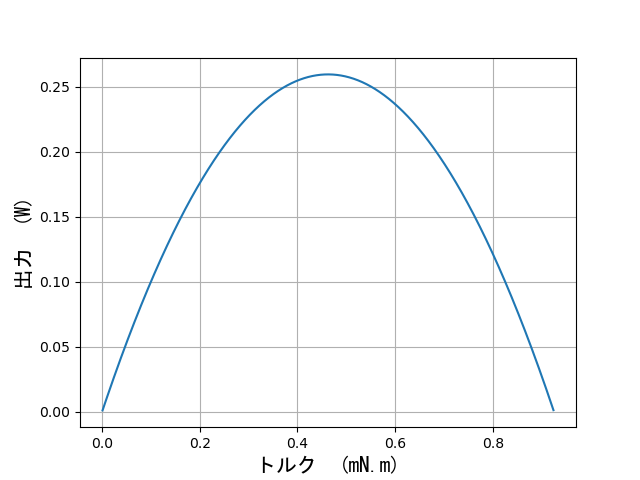
\includegraphics[width=7cm]{./Image/output.png}
% 	\caption{「負荷トルク $\times$ 出力」グラフ}
% 	\label{fig:output}
% \end{figure}
\subsection{モータ特性表生成}\label{sub:}
\ref{sub:mortortoku}節と、\ref{sub:toku_gurahu}節で生成した合計5つの画像を、ライブラリreportlab(表\ref{tab:libr}参照)を用いて、PDFファイルに書き込み、モータ特性表を生成する。
モータ特性表のPDFファイルのファイル名は、「characteristicTable.pdf」で生成する。同じファイル名がある場合、上書き保存する。
この処理で生成するモータ特性表を、図\ref{fig:tokuseihyou}に示す。
\begin{figure}[t]
	\centering
	\fbox{
	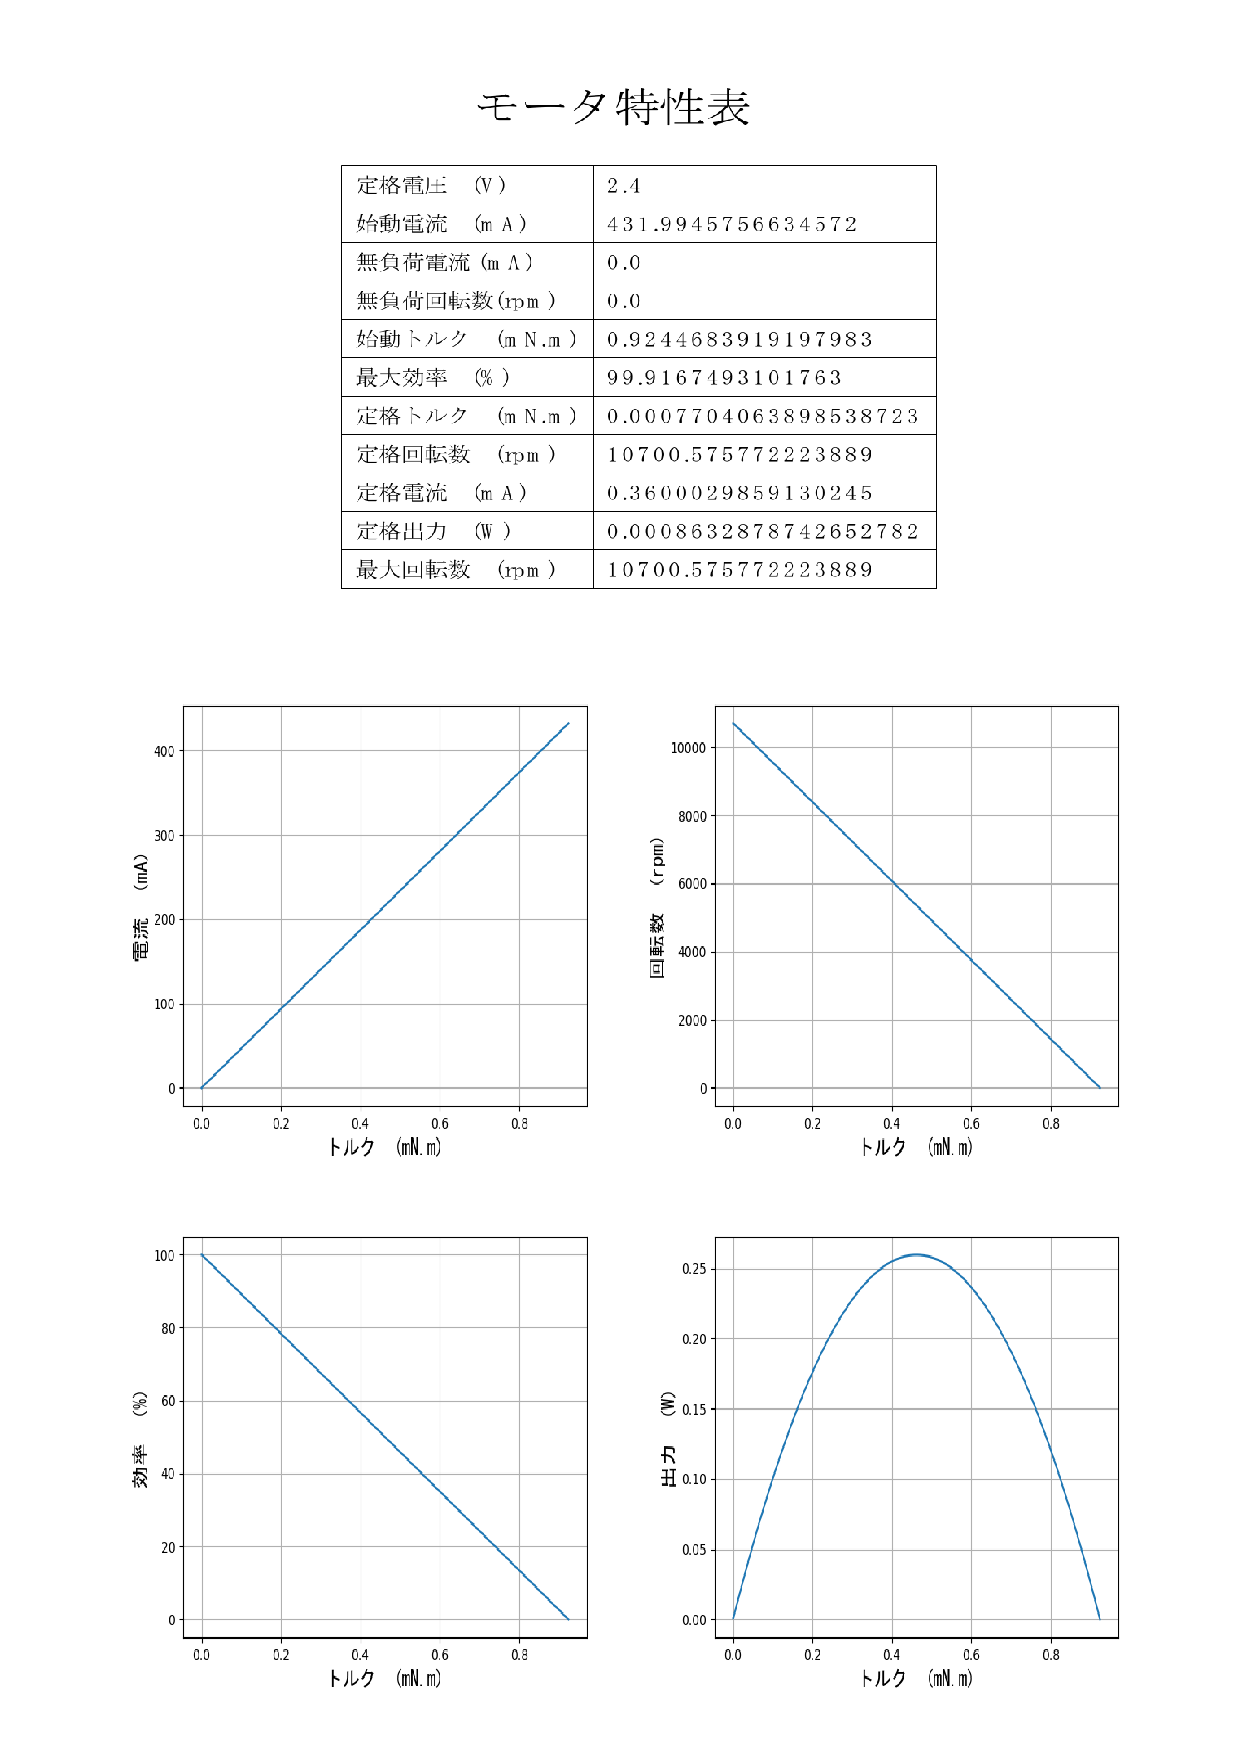
\includegraphics[width=16cm,pagebox=cropbox]{Image/characteristicTable.pdf} 
	}
	\caption{モータ特性表}
	\label{fig:tokuseihyou}
\end{figure}
% \chapter{機能}\label{cha:Function}

本章では、本研究で試作したモータ特性表自動生成ツールの機能について説明する。\\

モータ特性表自動生成ツールは、OpenModelicaでモータのモデルをシミュレーションした時に出力される
csvファイルを読み込み、実行することによって、モータ特性表を生成する。\\

\section{対応するモデル}\label{taioumodel}
今回試作したモータ特性表自動生成ツールでは以下のModelicaモデルのシミュレーション結果に対応する。
\begin{itemize}
	\item モータ単体のモデル
	\item モータ単体のモデルを一つに統一したモデルを使用するモデル
\end{itemize}
なお、今回はモータの中でもブラシ付きDCモータに対応する。\\
以降、上記のモデルについて具体的に説明する。

\subsection{モータ単体のモデル}\label{sec:sub1}
モータ単体のモデルとは、電源部品、抵抗部品、インダクター部品、起電力部品、慣性部品、接地部品の
OpenModelicaでブラシ付きDCモータについてシミュレーションするために、最低限必要となる部品を持つモデルのことである。\\
上記6つの部品が必要な理由は、ブラシ付きDCモータの等価回路\cite{等価回路}をModelicaで表す際に
使用する部品\cite{modelicaシステム本}だからである。\\
ブラシ付きDCモータの等価回路を図\ref{fig:touka}に、モータ単体のモデルを図\ref{fig:tantai_model}に、
モータ単体のモデルをModelicaコードで表したものを図\ref{fig:tantai_modelica}に示す。

\begin{figure}[t]
	\centering
	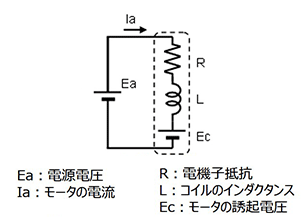
\includegraphics[width=10cm]{./Image/touka.png}
	\caption{等価回路}
	\label{fig:touka}
  \end{figure}

\begin{figure}[t]
  \centering
  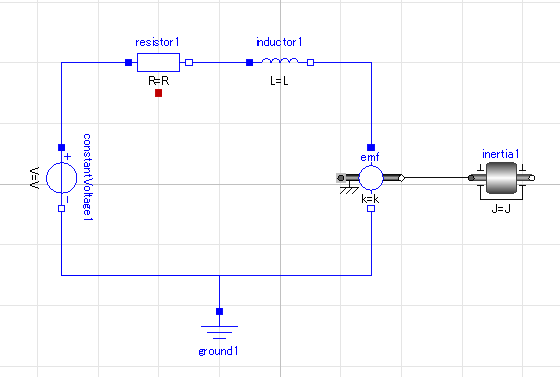
\includegraphics[width=10cm]{./Image/tantai_model.png}
  \caption{モータ単体のモデル}
  \label{fig:tantai_model}
\end{figure}

\begin{figure}[t]
	\centering
	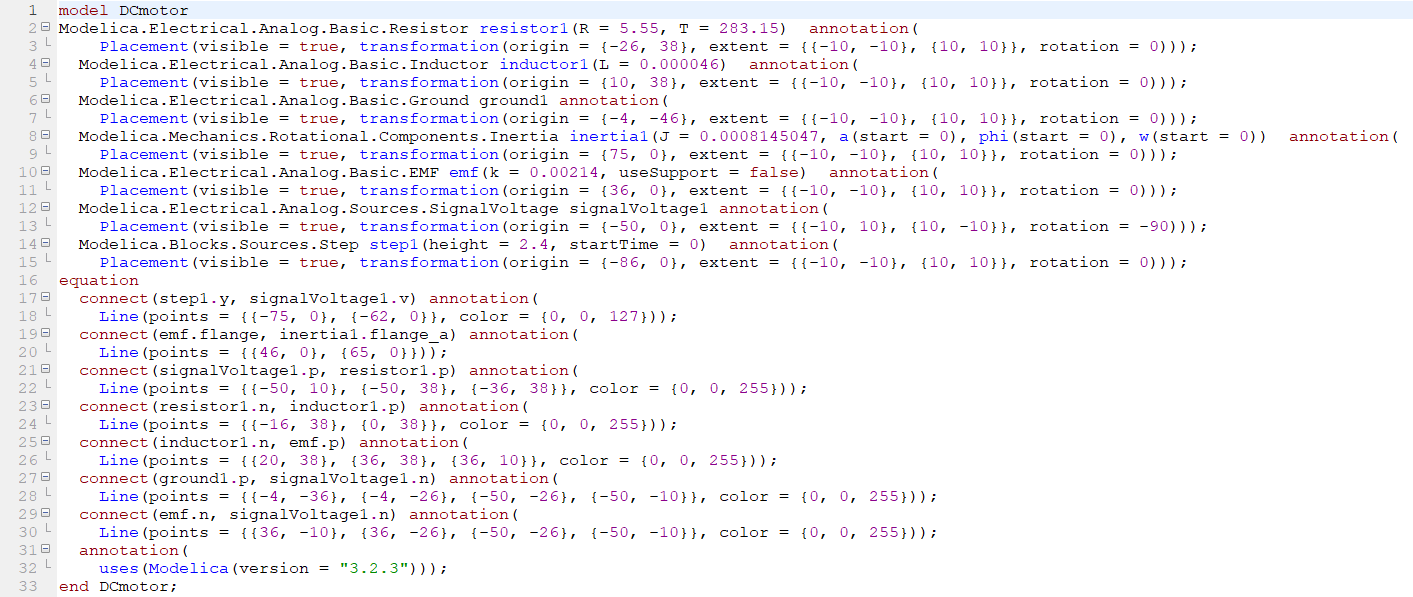
\includegraphics[width=16.5cm,height=8cm]{./Image/tantai_modelica.png}
	\caption{モータ単体のモデルのModelicaコード}
	\label{fig:tantai_modelica}
  \end{figure}

\subsection{モータ単体のモデルをサブシステムとするモデル}\label{sec:sub2}
モータ単体のモデルをサブシステム\cite{modelicaシステム本}(準備に書く?)とするモデルとは、\ref{sec:sub1}節で説明した
モータ単体のモデルを一つのモデルにして、サブシステムとして書いたモデルのことである。


\section{特性表生成}\label{kenkyu_mokuteki}
今回試作したモータ特性表自動生成ツールには次の~~~個の機能がある。

\begin{itemize}
	\item are
	\item sore 
\end{itemize}

\subsection{特性表生成機能}\label{sec:tokusei}
特性表生成機能は、以下の要素を持つモータ特性表を生成する。


% \chapter{実装}\label{cha:Implementation}

\section{シミュレーション結果解析機能}\label{kyap_re}

\section{特性表生成機能}\label{gazou_input}

\chapter{適用例}\label{cha:Indication}
本章では、本研究で作成した


\section{モータ単体のモデル}


\section{モータ単体のModelicaモデルをサブシステムとするモデル}

\chapter{考察}\label{cha:Discussion}
本論文では、性能を決定付ける特定の値を確認するためにかかる時間の削減を目的として、モータ特性表自動生成ツールを試作した。

なお、本研究では、シミュレーションの対象として、ブラシ付きDCモータを対象とする。

4章において、本論文で試作したモータ特性表自動生成ツールに、ブラシ付きDCモータのModelicaモデルと、
ブラシ付きDCモータのModelicaモデルをサブシステムとするモデルの2つが出力するcsvファイルを適用した。
その結果、本論文で試作したモータ特性表自動生成ツールが正しく動作することを確認できた。以下に、本論文で試作したモータ特性表自動生成ツールについて考察する。
\section{評価}

\subsection{評価方法}
% \todo{下記のコマンドを書き換える!}
% \newcommand{\mExist}{既存の手法}
% \newcommand{\mExtend}{本研究の手法}
% \newcommand{\mInput}{仕様書}
% \newcommand{\mOutput}{仕様書}

% \mExist{}と、\mExtend{}で、作成(生成)に要した時間の比較検証を行った。
% その結果を、表\ref{tab:time}に示す。

% 対象とした\mInput{}は、\ref{cha:domain}節で用いた コード\ref{fig:vdm_park}である。
% \mOutput{}を作成する時間を計測した。
% 生成する\mOutput{}としては、以下を基準とした。\todo{なにをもって完成かを書く!}
% \begin{enumerate}
%   \item onポイント、offポイント、inポイント、outポイントを出力(記述)する
%   \item onポイント、offポイント、outポイントには、着目条件式も出力(記述)する
%   \item offポイントには、着目変数も出力(記述)する
%   \item 各ポイントには、期待出力と正常系であるかどうかも出力(記述)する
% \end{enumerate}

% 検証に参加したメンバーは本研究室の大学院生\todo{X}人と学部4年生\todo{Y}人であり、
% 普段からソースコードの読み書きを行い、基本的なプログラミングの知識を有している。
% \mInput{}の知識を持たない者も含まれるが、
% 今回の検証に必要な文法は、事前に他の\mInput{}の例を用いてレクチャーした。
% また、\mOutput{}生成についても、事前に他の\mInput{}と\mOutput{}の例を用いてレクチャーした。

% 人手による検証では、
% コード\ref{fig:vdm_park}を印刷した紙を渡し、
% \mInput{}を確認後、
% \mOutput{}を書き始めてから、\mOutput{}を記述し終えるのに要した時間を計測した。
% \todo{なんか}が不正確な場合、間違いを指摘し、
% 被験者が正しい\mOutput{}を記述した時点で時間計測終了とした。
% また、制限時間を\todo{Z}分とし、制限時間を超えた場合、その場で時間計測終了とした。

% \mExtend{}による検証では、
% \todo{計測はじめから終わりの条件と、使ったPCの仕様を書く}
% コマンドライン上での命令操作で、\mExtend{}による\mOutput{}生成を行うのに要した時間を計測した。
% また、実験に用いたコンピュータは、OS:Windows10 Pro、CPU:3.6GHz Intel Core i7、メモリ:16GBである。

% \todo{純粋な、実行時間を書く}
% なお、JavaのSystem.nanoTime\cite{nanotime}メソッドを用いて、
% 命令操作を省いた純粋な\mOutput{}生成処理に\mExtend{}が要した時間を計測した結果、
% \todo{A}秒であった。

% 人手による作成と比較した結果、平均で\todo{B}分程の時間短縮を確認できた。
% 対象にした\mInput{}には、\todo{なにか}独特の文法等は含まれないため、
% \todo{なにか}に対する慣れなどの影響は無視できるものと思われる。
% また、人手による\mOutput{}生成の場合、ヒューマンエラーも見られた。
% \todo{ヒューマンエラーがあったら、具体例を書く}
% 具体的には、offポイントの記述時に、条件式の解釈を間違え、誤った期待出力を記述してしまった。(例:入力(17、 20)の期待出力を``遊園地チケットは割引価格とならない。(妻の年齢 $<$ 16)''と記述した。)
% \mInput{}の規模が拡大すると、人手とコンピュータとの処理効率の差に加えて、
% ヒューマンエラーの有無などにより、\mOutput{}生成に要する時間の差は更に拡大していくと思われる。
% 以上から、\mExtend{}は有用性が向上したと考える。

% % \begin{table}[tp]
% % \centering
% % \caption{コード\ref{fig:vdm_park}の\mOutput{}作成に要した時間の比較}
% % \label{tab:time}
% % \begin{tabular}{cc}
% % \begin{minipage}[c]{0.5\hsize}
% %   \centering
% %   \begin{tabular}{c|c}
% %     被験者  & 時間              \\
% %     \hline
% %     \hline
% %     被験者A & 8m 16s            \\ \hline
% %     被験者B & 10m 23s           \\ \hline
% %     被験者C & 30m(制限時間超過) \\ \hline
% %     被験者D & 24m 04s
% %   \end{tabular}
% % \end{minipage} &
% % \begin{minipage}[c]{0.5\hsize}
% %   \centering
% %   \begin{tabular}{c|c}
% %                  & 時間    \\
% %     \hline
% %     \hline
% %     被験者(平均) & 18m 10s \\ \hline
% %     BWDM         & 0m 15s
% %   \end{tabular}
% % \end{minipage}
% % \end {tabular}
% % \end{table}

本論文で試作したモータ特性表自動生成ツールの有用性を評価するため、本研究室の学部4年生4人に対して、実験を行い、特定の値を確認するためにかかる時間を削減できたかどうかを検証する。
実験には、内容が異なる2つのシミュレーション結果のファイルを用いた。これらのファイルをそれぞれ「ファイルA」、「ファイルB」と定義する。

実験方法は、ケースXとケースYに分けて行う。

ケースXでは、ファイルAに対して、モータ特性表自動生成ツールを使用せず、表計算ソフトを用いて問題に回答してもらう。次に、ファイルBに対して、モータ特性表自動生成ツールを使用して問題に回答してもらう。

ケースYでは、ファイルBに対して、モータ特性表自動生成ツールを使用せず、表計算ソフトを用いて問題に回答してもらう。次に、ファイルAに対して、モータ特性表自動生成ツールを使用して問題に回答してもらう。

ケースXとケースY で出題する問題を、図\ref{fig:mondai}に示す。

この問題を解答するのに要する時間を測定することにより、モータ特性表自動生成ツールを用いることで、特定の値を確認するためにかかる時間を削減できるかどうかを検証する。

被験者4名を2つのグループに分け、片方のグループに「ケースX」の実験を行い、もう片方のグループに「ケースY」の実験を行った。

「ケースX」の実験結果を、表\ref{resultX}に、「ケースY」の実験結果を表\ref{resultY}にそれぞれ示す。

\begin{figure}[t]
	\centering
	\fbox{
	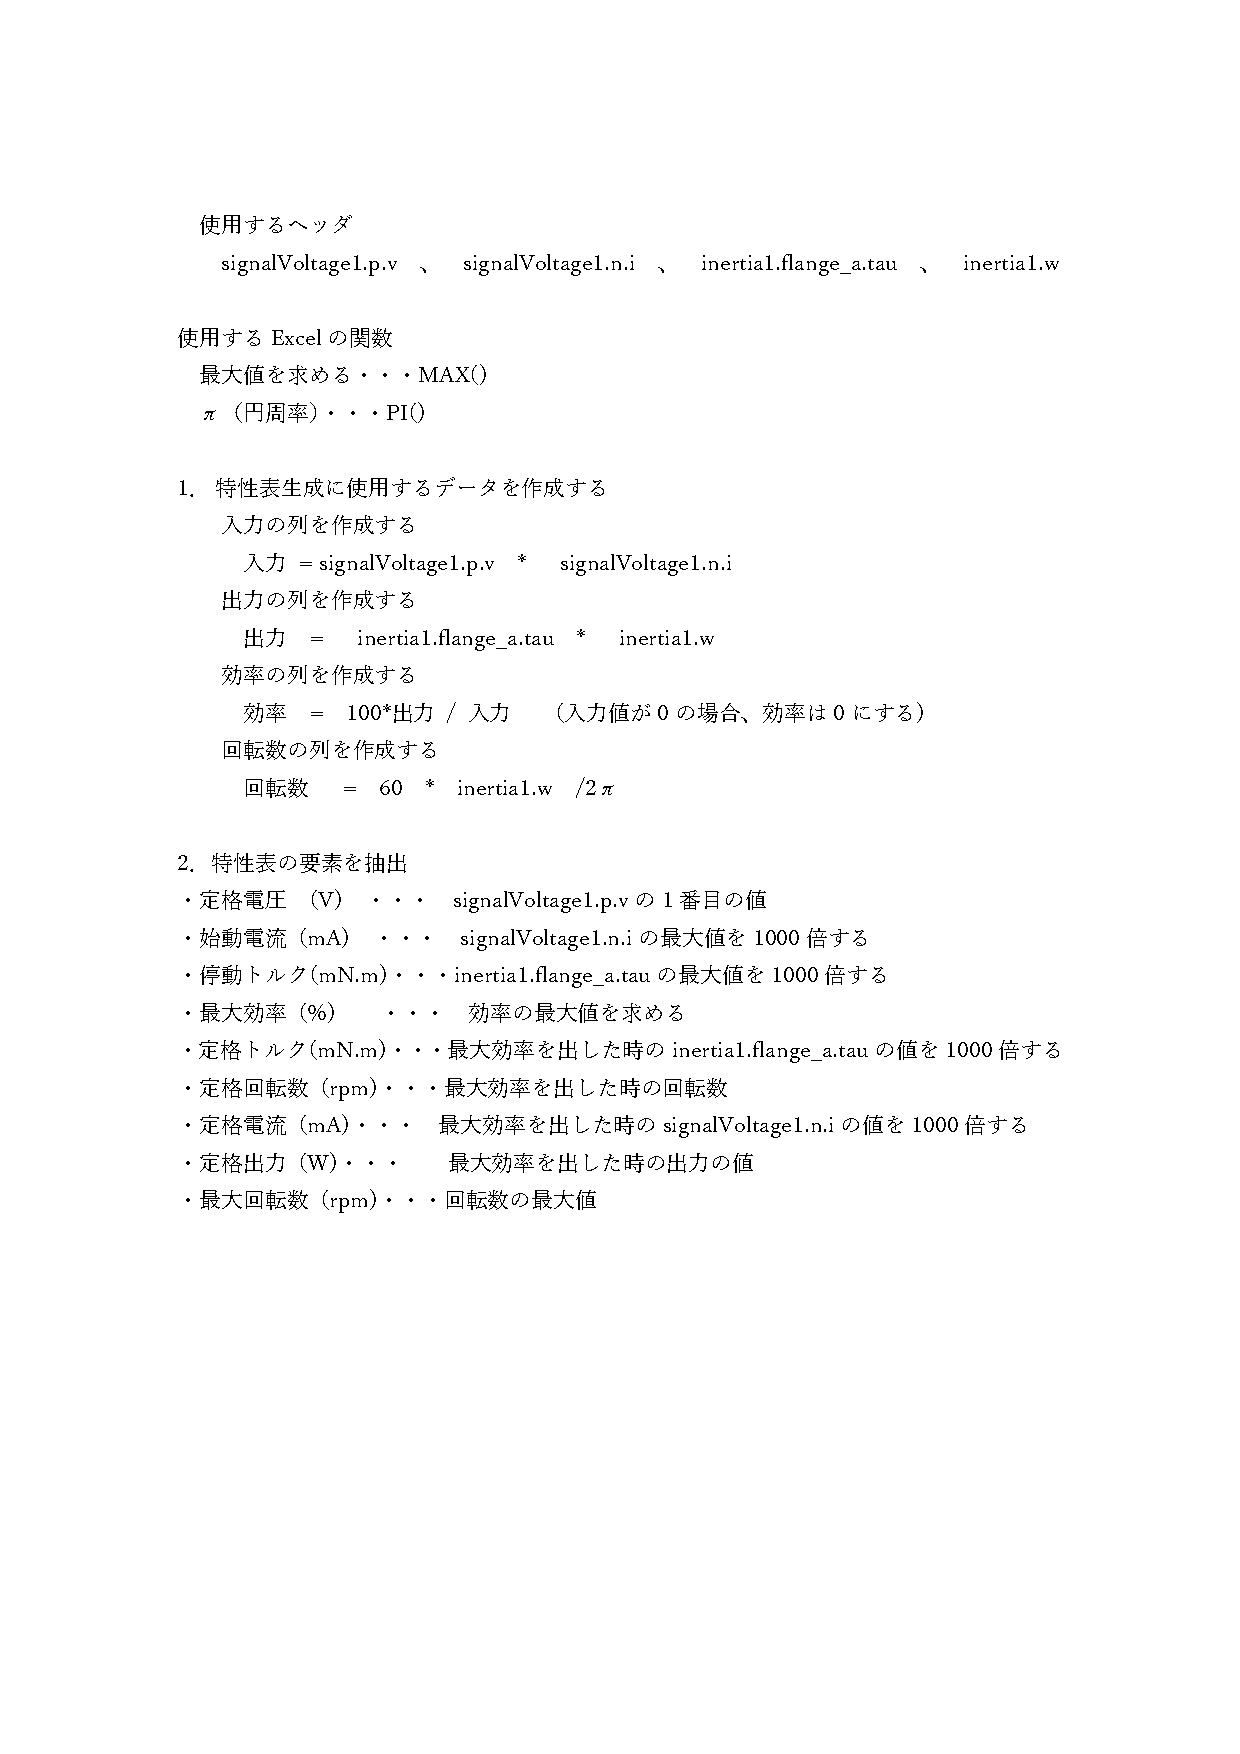
\includegraphics[width=16cm,pagebox=cropbox]{Image/実験方法の説明.pdf}
	}
	\caption{ケースXとケースY で出題する問題}
	\label{fig:mondai}
\end{figure}

\begin{table}[tp]
  \begin{center}
    \caption{ケースXの実験結果}
    \label{resultX}
    \begin{tabular}{c|c|c|c|c|}
    \cline{2-5}
                              & \multicolumn{2}{c|}{ツール未使用} & \multicolumn{2}{c|}{ツール使用} \\ \hline
    \multicolumn{1}{|c||}{被験者} & 回答時間           & 正答率          & 回答時間           & 正答率         \\ \hline\hline
    \multicolumn{1}{|c||}{1}   & 13分5秒           & 56\%         & 57秒           & 100\%         \\ \hline
    \multicolumn{1}{|c||}{2}   & 14分50秒          & 67\%          & 1分20秒          & 100\%         \\ \hline\hline
    \multicolumn{1}{|c||}{平均}   & 13分57.5秒          & 61.5\%          & 1分8.5秒          & 100\%         \\ \hline
    \end{tabular}
  \end{center}
\end{table}

\begin{table}[tp]
  \begin{center}
    \caption{ケースYの実験結果}
    \label{resultY}
    \begin{tabular}{c|c|c|c|c|}
    \cline{2-5}
                              & \multicolumn{2}{c|}{ツール未使用} & \multicolumn{2}{c|}{ツール使用} \\ \hline
    \multicolumn{1}{|c||}{被験者} & 回答時間           & 正答率          & 回答時間           & 正答率         \\ \hline\hline
    \multicolumn{1}{|c||}{3}   & 21分35秒           & 67\%         & 1分10秒           & 100\%         \\ \hline
    \multicolumn{1}{|c||}{4}   & 18分6秒          & 100\%          & 1分58秒          & 89\%         \\ \hline\hline
    \multicolumn{1}{|c||}{平均}   & 19分50.5秒          & 83.5\%          & 1分34秒          & 94.5\%         \\ \hline
    \end{tabular}
  \end{center}
\end{table}

「ケースX」の実験結果から、モータ特性表自動生成ツールを用いない場合の解答時間の平均は「13分57.5秒」である。また、正答率の平均は「61.5\%」である。
一方、モータ特性表自動生成ツールを用いた場合の解答時間の平均は「1分8.5秒」である。また、正答率の平均は「100\%」である。

この結果から、「ケースX」の実験においてモータ特性表自動生成ツールを用いた場合、解答時間の平均は用いなかった場合に比べて「91.8」\%削減できた。
また、モータ特性表自動生成ツールを用いた場合の方が、用いなかった場合に比べて正答率が高いことが示せた。

「ケースY」の実験結果から、モータ特性表自動生成ツールを用いない場合の解答時間の平均は「19分50.5秒」である。また、正答率の平均は「83.5\%」である。
一方、モータ特性表自動生成ツールを用いた場合の解答時間の平均は「1分34秒」である。また、正答率の平均は「94.5\%」である。

この結果から、「ケースY」の実験においてモータ特性表自動生成ツールを用いた場合、解答時間の平均は用いなかった場合に比べて「92.1」\%削減できた。
また、モータ特性表自動生成ツールを用いた場合の方が、用いなかった場合に比べて正答率が高いことが示せた。


これらの結果により、モータ特性表自動生成ツールを用いることで、特定の値を確認するためにかかる時間を削減できることを確認した。
また、モータ特性表自動生成ツールを用いることで、正答率が上がったことを確認できた。正答率が上がった理由として、モータ特性表自動生成ツールを用いることにより、人手によるミスを削減できたことが考えられる。
具体的には、モータ特性表自動生成ツールを用いない場合、手動で表計算ソフトから特定の値を抽出し、計算を行う必要があるため、この過程においてミスが発生する可能性が高まったことが考えられる。
一方、モータ特性表自動生成ツールを用いた場合、ツールが自動で特性表を生成し、提示することにより、人手によるミスが発生する可能性を削減できたことが考えられる。

以上の結果により、モータ特性表自動生成ツールの有用性があることを示せた。また、モータ特性表自動生成ツールを用いることで、特定の値を確認する際に生じるミスを削減できることが確認できた。


\subsection{結果}
本論文で試作したモータ特性表自動生成ツールは、

\section{関連研究}
関連研究について考察する。

\subsection{MATLABとの比較}
モデルベースシステム開発で使用されるツールとして、OpenModelicaの他に、MATLABがある。
MATLABはMathWorks社が開発する科学技術計算用のプログラミング言語である。
MATLABは、制御システム、信号処理、ディープラーニングなど幅広い分野の科学技術計算ができる。
また、ブロック線図シミュレータであるSimulinkと連携させることで、モータのモデル化、シミュレーション、グラフの描画ができる。
しかし、モータの性能を決定づける値の算出や、グラフの描画はできるが、モータの特性表の自動生成はできない。
一方、本研究で試作したモータ特性表自動生成ツールは、OpenModelicaのシミュレーション結果から、モータ特性表を自動生成できる。
このため、特性表と特性グラフをまとめたモータ特性表を自動生成できることが試作したツールの利点といえる。


\subsection{JMAG-Express Onlineとの比較}
\begin{table}[t]
	\centering
	\caption{本研究で試作したモータ特性表自動生成ツールにおけるモータ特性表出力までの実行時間}
	\begin{tabular}{|c|c|} \hline
	  ファイルサイズ(KB) & 実行時間(s)\\ \hline \hline
	  37 & 0.884 \\ \hline
	  47 &  0.978\\ \hline
	  2,909 &  1.024 \\ \hline
	  3,569 & 1.025 \\ \hline
	  5,496 &  1.078\\ \hline
	  71,987 &  3.329 \\ \hline
	\end{tabular}
	\label{tab:executionTime}
  \end{table}

パラメータベースのモータ設計支援ツールとして、JSOL社が開発するJMAG-Express Online(以下JMAG)がある\cite{jmag}。
JMAGは、形状テンプレート、材料、巻線および駆動条件のパラメータを入力することで、
モータ特性表(特性表と特性グラフ)を生成することができる。
さらに、モータ特性表に出力する基本特性(トルク、回転数など)は1秒程度で計算できる。
しかし、パラメータベースのモータ設計支援ツールであるため、
モデルベースシステム開発の利点である柔軟な開発が、JMAGを利用できない。
一方、本研究で試作したモータ特性表自動生成ツールは、OpenModelicaのシミュレーション結果から、
モータ特性表を自動生成できる。
ここで、本研究で試作したモータ特性表自動生成ツールにおけるモータ特性表出力までの実行時間を、表\ref{tab:executionTime}にそれぞれ示す。
表\ref{tab:executionTime}が示すように、試作したツールも1秒程度でモータ特性表に出力する基本特性を計算できるため、JMAGと同程度の時間で、モータ特性表を生成できる。
このため、モータをモデルベースシステム開発手法で開発する際に、試作したツールを用いてモータの性能を確認できることが、試作したツールの利点といえる。

\section{ツールの問題点}

以下に、今回作成したモータ特性表自動生成ツールの問題点を示す。

\begin{itemize}
	\item 対象とするモータのモデルが1種類しかない\\
      本論文で試作したモータ特性表自動生成ツールが対象とするのはブラシ付きDCモータである。しかし、ブラシレスモータやACモータなどには対応していない。
      そのため、それらを用いた回路のシミュレーション結果からモータ特性表を作成できない。
		  この問題点は、新たに対象とするモータのcsvファイルを解析し、特性表の要素を算出できるようにすることで、解決できると考える。

  \item 特性表の要素をユーザが変更できない\\
        本論文で試作したモータ特性表自動生成ツールが生成する特性表は、12個の要素を持つ。
        しかし、ユーザがこの要素を変更することはできない。
        この問題点は、ユーザが特性表の要素を設定できるようにすることで、解決できると考える。

  \item 特性グラフを出力形式をユーザが指定できない\\
        本論文で試作したモータ特性表自動生成ツールは、4つの特性グラフを個別に出力する。
        しかし、特性グラフは1つのグラフに複数の要素を表示することで、グラフの比較を行いやすくなる。
        そのため、特性グラフの出力形式をユーザが指定できるようにすることで、グラフの比較がしやすくなり、 本論文で試作したモータ特性表自動生成ツールの有用性が向上すると考える。


\end{itemize}








\chapter{おわりに}\label{cha:Conclusion}


以下に、今後の課題を示す。





%% listings-modelica.cfg
%% Copyright 2014 Martin Sjoelund, Dietmar Winkler
%
% This work may be distributed and/or modified under the
% conditions of the LaTeX Project Public License, either version 1.3
% of this license or (at your option) any later version.
% The latest version of this license is in
%   http://www.latex-project.org/lppl.txt
% and version 1.3 or later is part of all distributions of LaTeX
% version 2005/12/01 or later.
%
% This work has the LPPL maintenance status `maintained'.
%
% The Current Maintainer of this work is Dietmar Winkler
%
% Code repository https://github.com/modelica-tools/listings-modelica
%
% This work consists of the file listings-modelica.cfg

\lstdefinelanguage{modelica}
{
  morekeywords=[1]{
    algorithm,and,annotation,as,assert,block,break,case,class,connect,connector,
    constant,constrainedby,der,discrete,each,else,elseif,elsewhen,encapsulated,
    end,enumeration,equality,equation,expandable,extends,external,failure,final,
    flow,for,function,guard,if,import,in,initial,inner,input,List,local,loop,
    match,matchcontinue,model,not,operator,Option,or,outer,output,package,parameter,
    partial,protected,public,record,redeclare,replaceable,return,stream,
    subtypeof,then,Tuple,type,uniontype,when,while},
  morekeywords=[2]{true, false},
  % Do not make true,false keywords because fn(true,x, false ) shows up as fn(true,x, *false*)
  morekeywords=[3]{optimization,constraint}, % Optimica keywords
  morekeywords=[4]{objective,startTime,finalTime,initialGuess},
  sensitive=true,
  comment=[l]//,
  morecomment=[s]{/*}{*/},
  alsodigit={.,-},
  morestring=[b]',
  morestring=[b]",
}[keywords,comments,strings]

\definecolor{keywordcolor1}{rgb}{0,0,.4}
\definecolor{keywordcolor2}{rgb}{.90,0,0}
\definecolor{keywordcolor3}{rgb}{.4,0,.8}
\definecolor{keywordcolor4}{rgb}{0.5,0,0.5}
\definecolor{stringcolor}{rgb}{0.133,0.545,0.133}
% \definecolor{listingbgcolor}{rgb}{0.95,0.95,0.95}

\lstset{
  breaklines=true,
  language=modelica,
  basicstyle=\ttfamily,
  keywordstyle=[1]\color{keywordcolor1}\bfseries,
  keywordstyle=[2]\color{keywordcolor2},
  keywordstyle=[3]\color{keywordcolor3}\bfseries,
  keywordstyle=[4]\color{keywordcolor4},
  stringstyle=\color{stringcolor},
%  backgroundcolor=\color{listingbgcolor},
  framexleftmargin=5pt,
  xleftmargin=5pt,
  xrightmargin=5pt,
  showstringspaces=false
}

\newcommand{\code}[1]{\lstinline|#1|}
\newcommand{\modelica}[1]{\lstinline[language=modelica]|#1|}

%%
% 謝辞
%
\acknowledgment


%%
% 参考文献
%

\bibliography{bibtex} %bibファイルの.bibの前の部分


\bibliographystyle{junsrt} %引用された順番に出力

% \newpage
% \listoftodos
\end{document}